
\section{1次元調和振動子ポテンシャル}
$x$軸上で原点からの距離に比例する引力を受けて単振動する粒子について考える。
この時の粒子のポテンシャルエネルギーは角振動数$\omega$を用いて、$V(x) = \dfrac{1}{2}m\omega x^2$とかける。
よって、ポテンシャルは位置にのみ依存するので、時間に依存しないシュレディンガー方程式を用いて

\begin{equation}
	\label{harmony_schrodinger_eq}
	E\psi(x) = - \dfrac{\hbar^2}{2m} \dfrac{d^2 \psi(x)}{d x^2} + \dfrac{1}{2}m\omega x^2\psi(x)
\end{equation}

となる。このままでも解くことができるが、式を簡単にして見通しをよくしたい。
そのためには、
\begin{align}
		\label{xi}
		\xi &= \sqrt{\dfrac{m\omega}{\hbar}}x \\
		\label{eps}
		\epsilon &= \dfrac{2E}{\hbar\omega}
\end{align}
という、無次元の変数$\xi$、$\epsilon$を導入する。

(\ref{harmony_schrodinger_eq})の両辺に$\dfrac{2}{\hbar\omega}$をかけると、

\begin{equation}
	\dfrac{2E}{\hbar\omega}\psi(x) = - \dfrac{\hbar}{m\omega} \dfrac{d^2 \psi(x)}{d x^2} + \dfrac{m\omega}{\hbar} x^2\psi(x)
\end{equation}

変形して、
\begin{equation}
	\dfrac{2E}{\hbar\omega}\psi(x) = - \dfrac{d^2 \psi(x)}{d \dfrac{m\omega}{\hbar} x^2} + \dfrac{m\omega}{\hbar} x^2\psi(x)
\end{equation}
(\ref{xi})、(\ref{eps})より、
\begin{equation}
	\epsilon\psi(\xi) = - \dfrac{d^2 \psi(\xi)}{d \xi^2} + \xi^2\psi(\xi)
\end{equation}
よって、
\begin{equation}
	\label{harmony_DE}
	\dfrac{d^2 \psi(\xi)}{d \xi^2} + (\epsilon - \xi^2)\psi(\xi) = 0
\end{equation}
となる。
この微分方程式を解けば良いのだが、これが難しい。
上手い具合に近似できないか考えてみる。
$\xi \to \pm \infty$では$\epsilon$は$\xi$に比べて小さいので無視できそうだ。
すると、
\begin{equation}
	\dfrac{d^2 \psi(\xi)}{d \xi^2}  - \xi^2\psi(\xi) = 0
\end{equation}
これは簡単に解く事ができて、
\begin{equation}
	\psi(\xi) = He^{\pm \frac{\xi^2}{2}}
\end{equation}
となる。($H$は任意定数)
$\xi \to \pm\infty$の極限では波動関数$\psi$は収束しなければいけない。
そのため、指数部分の符号は負である必要がある。よって、
\begin{equation}
	\psi(\xi) = He^{-\frac{\xi^2}{2}}
\end{equation}
これは、$\xi \to \pm \infty$の極限を仮定した解であることに注意しなければならない。
実際に、これを(\ref{harmony_DE})に戻してみると、当然解になっていない事が確認できる。
この解を元に$\xi \to \pm \infty$の極限以外でも成立するような解を探す。
では、どうすれば良いのかというと、定数$H$が実は$\xi$の関数$H(\xi)$であると仮定する上手く行く。

今、
\begin{equation}
	\psi(\xi) = H(\xi)e^{-\frac{\xi^2}{2}}
\end{equation}

これを(\ref{harmony_DE})に戻す。
積の微分であることに注意すると、
\begin{equation}
	\dfrac{d\psi(\xi)}{d\xi} = e^{-\frac{\xi^2}{2}}\dfrac{dH(\xi)}{d\xi} - \xi H(\xi)e^{-\frac{\xi^2}{2}}
\end{equation}
\begin{equation}
	\dfrac{d^2\psi(\xi)}{d\xi^2} = e^{-\frac{\xi^2}{2}}\dfrac{d^2 H(\xi)}{d\xi^2} -2\xi e^{-\frac{\xi^2}{2}}\dfrac{dH(\xi)}{d\xi}
	 															+ (\xi^2 - 1)H(\xi)e^{-\frac{\xi^2}{2}}
\end{equation}

なので、(\ref{harmony_DE})に戻すと、

\begin{equation}
	\label{H_DE}
	\left[\dfrac{d^2}{d\xi^2} -2\xi\dfrac{d}{d\xi} + (\epsilon -1)\right]H(\xi) = 0
\end{equation}

この微分方程式を解くことになる。
これを解くために、$H(\xi)$が級数展開できると仮定する。
\begin{equation}
	H(\xi) = \sum_{k=0}^{\infty}a_k \xi^k
\end{equation}
この$a_k$を求める事ができれば、$H(\xi)$が決まるので、微分方程式が解けたことになる。
微分すると、
\begin{equation}
	\dfrac{d H(\xi)}{d\xi} = \sum_{k=1}^{\infty}a_k k\xi^{k-1} = \sum_{k=0}^{\infty}a_k k\xi^k
\end{equation}
\begin{equation}
	\dfrac{d^2 H(\xi)}{d\xi} = \sum_{k=2}^{\infty}a_k k(k-1)\xi^{k-2} = \sum_{k=0}^{\infty}a_{k+2} (k+2)(k+1)\xi^k
\end{equation}
よって、(\ref{H_DE})に戻すと、
\begin{equation}
	\sum_{k=0}^{\infty} \left[ (k+2)(k+1)a_{k+2} - (2k - \epsilon + 1)a_k  \right] \xi^k = 0
\end{equation}
これより、
\begin{equation}
	(k+2)(k+1)a_{k+2} = (2k - \epsilon + 1)a_k
\end{equation}
という事がわかるので、
\begin{equation}
	\label{recurrence_relation_1}
	a_{k+2} = \dfrac{(2k - \epsilon + 1)}{(k+2)(k+1)}a_k
\end{equation}
となり、
\begin{itemize}
	\item $a_0$が決まれば、偶数次の項
	\item $a_1$が決まれば、奇数次の項
\end{itemize}
が決まることになる。

$H(\xi)$は無限級数である。その為、発散するのか収束するのか気になる。

$k \to \infty$の時、$a_{k+2} \approx \dfrac{2}{k}a_k$と近似できる。
$k = 2n$とすると、$a_{2(n+1)} \approx \dfrac{1}{n}a_{2n}$となる。
なので、
\begin{equation}
	H(\xi) \approx \sum_{n}\dfrac{1}{n!}\xi^{2n} \approx e^{\xi^2}
\end{equation}
すると、
\begin{equation}
	\psi(\xi) = H(\xi)e^{-\frac{\xi^2}{2}} \approx e^{\frac{\xi^2}{2}}
\end{equation}
となり、$\xi \to \infty$で発散してしまう。
$H(\xi)$が無限級であるために発散してしまうのだ。
なので、収束させるために$H(\xi)$が有限個の項で終わるような条件を付けてやれば良い。
(\ref{recurrence_relation_1})より、
\begin{equation}
	\label{eps_requirement}
	\epsilon = 2n + 1
\end{equation}
とすれば、第$n$項は存在するが、第$n+2$項から$0$になる。
第$n+1$項も$0$であって欲しいので、
\begin{itemize}
	\item $n$が偶数 $\Rightarrow a_1 = 0$
	\item $n$が奇数 $\Rightarrow a_0 = 0$
\end{itemize}
という条件を付けて、$n$が偶数の時は奇数次の項が、$n$が奇数の時は偶数次の項が$0$になるようにしてしまえば良い。

$n$によって、$H(\xi)$が変わるので、$H_n(\xi)$と書くようにする。

いくつか計算してみると、
$$
\begin{aligned} H_{0}(\xi) &=a_{0} \\ H_{1}(\xi) &=a_{1} \xi \\ H_{2}(\xi) &=a_{0}\left(1-\frac{4}{1 \cdot 2} \xi^{2}\right) \\ H_{3}(\xi) &=a_{1}\left(\xi-\frac{4}{2 \cdot 3} \xi^{3}\right) \\ H_{4}(\xi) &=a_{0}\left(1-\frac{8}{1 \cdot 2} \xi^{2}+\frac{8}{1 \cdot 2} \frac{4}{3 \cdot 4} \xi^{5}\right) \\ & \vdots
\end{aligned}
$$

これの$H_n(\xi)$を{\bf エルミート(Hermite)多項式}と呼ぶ。

一般的に、エルミート多項式は
\begin{equation}
	H_{n}(\xi)=(-1)^{n} e^{\xi^{2}} \frac{\mathrm{d}^{n}}{\mathrm{d} \xi^{n}} e^{-\xi^{2}}
\end{equation}
と書ける。
いくつか計算してみると、
\begin{equation}
\begin{aligned}
	H_{0}(\xi) &= 1 \\
	H_{1}(\xi) &= 2 \xi \\
	H_{2}(\xi) &= 4 \xi^{2}-2 \\
	H_{3}(\xi) &= 8 \xi^{3}-12 \xi \\
						 & \vdots \end{aligned}
\end{equation}

$a_0$と$a_1$が$n$によって違うが、微分方程式(\ref{H_DE})を満たすので気にしなくて良い。

以上のことより、
\begin{equation}
	\label{harmony_psi}
	\psi_n(\xi) = H_n(\xi)e^{-\frac{\xi^2}{2}}
\end{equation}
と、(\ref{harmony_schrodinger_eq})を解く事ができた。

ここで、(\ref{eps})と、(\ref{eps_requirement})を思い出してみよう。
これらより、
\begin{equation}
	E_n = \hbar\omega(n+\frac{1}{2})
\end{equation}
$n$は$0$を含む正の整数である。(エルミート多項式を定義するため)

$n = 0$の時、$E_0 = \frac{1}{2}\hbar\omega$である。
つまり、調和振動子ポテンシャルでは、粒子の持つエネルギーは$0$にはならない。

エネルギーが$0$の状態は粒子が止まっていることを表す。
つまり、運動エネルギーが$0$であり、ポテンシャルエネルギーも$0$である。
ということは、運動量は$0$で、粒子は原点にあるという事がわかる。
位置と運動量が同時に確定してしまい、不確定性原理に反してしまう。
だから、エネルギーは$0$にはならない。

エネルギーが$0$にならないということは、このポテンシャルの中で粒子は振動をし続ける事になる。
位置と運動量を同時に確定させないためだ。
この、$n=0$の時の振動を{\bf 零点振動}と呼び、この時のエネルギー$E_0$のことを{\bf 零点エネルギー}と呼ぶ。

さて、(\ref{harmony_psi})より、波動関数を求める事ができたので、実際に波動関数の形を見てみよう。
固有エネルギー$En$と対応する波動関数$\psi_n$を$n=11$までplotしたものだ。
波動関数は固有エネルギー分を平行移動してあり、規格化されている。
\begin{figure}[htb]
	\begin{center}
		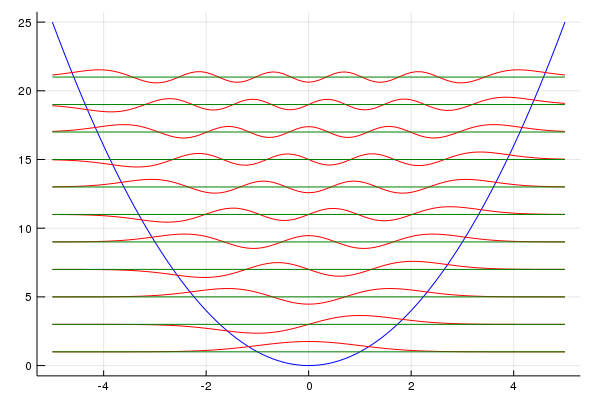
\includegraphics[height=6cm]{../fig/harmony.png}
		\caption{調和振動子ポテンシャルと波動関数($n=11$まで)}
		\label{}
	\end{center}
\end{figure}

量子的なミクロな世界にバネは存在しない。しかし、粒子が移動しようとしても元の位置に戻すような力、復元力が働くような状況を条件によっては作り出せるわけだ。
そのような復元力を級数展開して
\begin{equation}
	V(x) = a_0 + a_1 x + a_2 x^2 + a_3 x^3 + a_4 x^4 + \cdots
\end{equation}
と書けるとしよう。
$x$がとても小さい時、$3$次以降の項は$2$次の項に比べてほとんど無視できる程に小さい。
そして、$0$次と$1$次の項は$V(x) = a_2 x^2$を平行移動させる意味しかない。結局、考えるのは$2$次の項だけで十分であり、調和振動子ポテンシャルと同じ形になる。
なので、復元力によって粒子が振動しているような状況はこの調和振動子と同じ様な振る舞いになる。そのため、この調和振動子型ポテンシャルはとても重要なのだ。また、場合によっては$3$次や$4$次といった、高次の項を無視せずにもっと精密に解く場合はどうすれば良いのだろうか?それは摂動論を学ぶ必要がある。
